\section{随机动量方法}
\label{sec:sgdb-momentum}

小批量和控制变量都在改善单步的读数，代价是多读梯度或多存梯度。本节换一个问题：不增加读取，只把已经读过的梯度组合进当前方向，能得到什么，又要付出什么？

组合历史读数有两种效果。一致的成分累积起来，随机涨落互相抵消，这是平滑；旧读数来自旧的位置，当前梯度变化时方向跟不上，这是滞后。两者同时发生，而且历史进入了算法的状态，每一步的误差要连同历史一起分析。本节先讲当前点读数的重球法，再讲前瞻点读数的Nesterov方法，最后讲两种把动量做非线性变换的方法。

\subsection{随机重球法}
\label{sec:sgdb-heavy-ball}

\paragraph{主要思想}
第~\ref{chap:first-order-methods}章的重球法在当前梯度步之外，再加上一步历史位移。把其中的梯度换成当前点的随机读数$\hat{\bm g}^{(t)}$，就得到\term{随机重球法}（stochastic heavy ball method）。规定$\bm{x}^{(-1)}=\bm{x}^{(0)}$，
\begin{equation}
 \bm{x}^{(t+1)}=\bm{x}^{(t)}-\alpha\hat{\bm g}^{(t)}+\beta\bigl(\bm{x}^{(t)}-\bm{x}^{(t-1)}\bigr),\qquad 0\leq\beta<1.
 \label{eq:sgdb-hb}
\end{equation}

式~\eqref{eq:sgdb-hb}要存两个位置。实际计算常改写成只存一个速度向量$\bm{v}^{(t)}$的形式：取$\bm{v}^{(0)}=\bm{0}$，先更新速度，再更新位置，
\begin{equation}
 \bm{v}^{(t+1)}=\beta\bm{v}^{(t)}+\hat{\bm g}^{(t)},\qquad
 \bm{x}^{(t+1)}=\bm{x}^{(t)}-\alpha\bm{v}^{(t+1)}.
 \label{eq:sgdb-hb-velocity}
\end{equation}

两种写法等价。由速度形式，上一步的位移满足$\bm{x}^{(t)}-\bm{x}^{(t-1)}=-\alpha\bm{v}^{(t)}$，于是
\[
 -\alpha\bm{v}^{(t+1)}=-\alpha\hat{\bm g}^{(t)}-\alpha\beta\bm{v}^{(t)}
 =-\alpha\hat{\bm g}^{(t)}+\beta\bigl(\bm{x}^{(t)}-\bm{x}^{(t-1)}\bigr).
\]

还有第三种常见写法，把方向写成读数的移动平均。令$\bm{m}^{(t)}=(1-\beta)\bm{v}^{(t)}$，式~\eqref{eq:sgdb-hb-velocity}的速度递推两边乘以$1-\beta$，得到
\begin{equation}
 \bm{m}^{(t+1)}=\beta\bm{m}^{(t)}+(1-\beta)\hat{\bm g}^{(t)},\qquad
 \bm{x}^{(t+1)}=\bm{x}^{(t)}-\alpha'\bm{m}^{(t+1)},
 \label{eq:sgdb-hb-ema}
\end{equation}
其中两种写法的步长的对应关系是
\begin{equation}
 \alpha'=\frac{\alpha}{1-\beta}.
 \label{eq:sgdb-hb-effective}
\end{equation}

对应关系决定了调参的含义。在速度写法中固定$\alpha$而增大$\beta$，方向的总权重变大，$\alpha/(1-\beta)$随之变大，所以$\alpha/(1-\beta)$称为\term{有效步长}（effective step size）。在移动平均写法中固定$\alpha'$而增大$\beta$，方向的总权重不变，只是平均的窗口更长。比较两种实现时，先把参数换到同一种写法。

\paragraph{历史权重：平滑与滞后}
方向怎样由历史读数组成？反复代入速度递推，得到
\begin{equation}
 \bm{v}^{(t+1)}=\sum_{s=0}^{t}\beta^{t-s}\hat{\bm g}^{(s)}.
 \label{eq:sgdb-hb-weights}
\end{equation}

一个$s$轮之前的读数，权重是$\beta^{s}$，按等比衰减。移动平均写法中的权重是$(1-\beta)\beta^{s}$，全部加起来等于$1-\beta^{t+1}$，轮数足够多时接近$1$。图~\ref{fig:sgdb-momentum-track}(a)画出两个$\beta$对应的权重：$\beta$越接近$1$，权重越平，记忆越长。

\begin{BookInlineFigure}
  \centering
  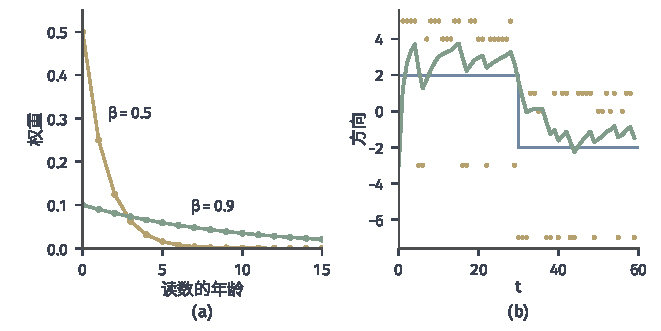
\includegraphics[width=112mm]{figures/05-optimization/05-stochastic-optimization/matplotlib/sgdb-momentum-track/figure.pdf}
  \caption{移动平均的平滑与滞后。(a)读数按年龄的权重$(1-\beta)\beta^{s}$，黄线$\beta=0.5$，绿线$\beta=0.9$。(b)蓝线是真实梯度，在$t=30$由$2$突变为$-2$；黄点是加上贯穿例噪声后的单次读数；绿线是$\beta=0.9$的移动平均方向（按权重之和归一化）。绿线的抖动比黄点小得多，但突变后要约十轮才转向。}
  \label{fig:sgdb-momentum-track}
\end{BookInlineFigure}

把两种效果算出来。先看平滑：设各轮读数的噪声相互独立，方差都是$\sigma^2$。移动平均的噪声部分是加权和，独立项的方差按权重平方相加，
\[
 (1-\beta)^2\sum_{s=0}^{t}\beta^{2s}\,\sigma^2
 =\frac{1-\beta}{1+\beta}\bigl(1-\beta^{2(t+1)}\bigr)\sigma^2 .
\]
于是轮数足够多时，方差缩小的倍数是
\begin{equation}
 \frac{1-\beta}{1+\beta}.
 \label{eq:sgdb-ema-noise}
\end{equation}

再看滞后：移动平均里读数的平均年龄是
\begin{equation}
 \sum_{s=0}^{\infty}s(1-\beta)\beta^{s}=\frac{\beta}{1-\beta}.
 \label{eq:sgdb-ema-age}
\end{equation}

取$\beta=0.9$，噪声方差缩小到约$0.053$倍，平均年龄却是$9$轮。图~\ref{fig:sgdb-momentum-track}(b)同时展示了两者：梯度不变时绿线紧贴真实值，梯度突变后绿线要约十轮才转向。这两个计算都假定噪声与位置无关，只说明趋势：真实运行中读数的位置本身受过去的噪声影响。

\paragraph{动量不是当前梯度的无偏估计}
读数条件无偏是说，固定历史后读数的均值等于当前梯度。动量方向并不继承这个性质。历史$\mathcal{F}^{(t)}$确定了$\bm{v}^{(t)}$，所以
\begin{equation}
 \mathbb{E}\bigl[\bm{v}^{(t+1)}\mid\mathcal{F}^{(t)}\bigr]=\beta\bm{v}^{(t)}+\bm{g}^{(t)},
 \label{eq:sgdb-hb-cond}
\end{equation}
只要$\bm{v}^{(t)}\neq\bm{0}$且$\beta>0$，它就不等于当前梯度$\bm{g}^{(t)}$。移动平均写法同样如此，条件均值是$\beta\bm{m}^{(t)}+(1-\beta)\bm{g}^{(t)}$。前面基于条件无偏的单步下降递推，不能把$\bm{v}^{(t+1)}$当成读数直接代入。

贯穿例给出具体的数。取$\alpha=0.1$，$\beta=0.5$，第一轮抽到第$3$项后位于$x^{(1)}=2.3$，速度是$v^{(1)}=-3$。此时三项梯度分别是$5.3,4.6,-2.1$，平均为$f'(2.3)=2.6$。第二轮的速度取$3.8$、$3.1$、$-3.6$三个值，条件均值是
\[
 \mathbb{E}\bigl[v^{(2)}\mid\mathcal{F}^{(1)}\bigr]=0.5\cdot(-3)+2.6=1.1\neq2.6.
\]

\paragraph{固定噪声下的稳态方差}
动量究竟能不能降低噪声的影响？在可以精确计算的情形中回答。考虑一元二次目标、加性噪声，下面的定理给出重球法长期的方差。

\begin{theorem}[加性噪声下重球法的稳态方差]
\label{thm:sgdb-hb-variance}
设$f(x)=\frac\lambda2x^2$，$\lambda>0$，读数为$\hat g^{(t)}=\lambda x^{(t)}+\xi^{(t)}$，其中$\xi^{(t)}$独立同分布，均值为零，方差为$\sigma^2$，且与此前的迭代独立。设$0\leq\beta<1$，$0<\alpha\lambda<2(1+\beta)$。则式~\eqref{eq:sgdb-hb}的迭代满足$\mathbb{E}x^{(t)}\to0$，并且
\begin{equation}
 \lim_{t\to\infty}\mathbb{E}\bigl[(x^{(t)})^2\bigr]
 =\frac{\alpha\sigma^2(1+\beta)}{\lambda(1-\beta)\bigl(2(1+\beta)-\alpha\lambda\bigr)}.
 \label{eq:sgdb-hb-variance}
\end{equation}
\end{theorem}

\begin{proof}
把式~\eqref{eq:sgdb-hb}写成二阶递推。令$a_1=1+\beta-\alpha\lambda$，$a_2=-\beta$，$s^2=\alpha^2\sigma^2$，则
\[
 x^{(t+1)}=a_1x^{(t)}+a_2x^{(t-1)}-\alpha\xi^{(t)}.
\]

特征方程是$r^2-a_1r-a_2=0$。条件$0\leq\beta<1$与$\lvert a_1\rvert<1+\beta$合起来保证两根都在单位圆内，这正是定理对$\alpha$和$\beta$的要求。所以均值的线性递推趋于零；二阶矩的线性递推的特征值是两根的两两乘积，也都在单位圆内，因而二阶矩收敛。记极限为
\[
 V_0=\lim_{t\to\infty}\mathbb{E}\bigl[(x^{(t)})^2\bigr],\qquad
 V_1=\lim_{t\to\infty}\mathbb{E}\bigl[x^{(t)}x^{(t-1)}\bigr].
\]

递推两边乘以$x^{(t)}$取期望。$\xi^{(t)}$与$x^{(t)}$独立且均值为零，噪声项消失；取极限得到$V_1=a_1V_0+a_2V_1$，也就是
\[
 V_1=\frac{a_1V_0}{1-a_2}.
\]

递推两边平方取期望，同样消去交叉项，取极限得到
\[
 V_0=(a_1^2+a_2^2)V_0+2a_1a_2V_1+s^2 .
\]

把$V_1$代入，两边乘以$1-a_2$并整理，$V_0$的系数变成
\[
 (1-a_2)(1-a_2^2)-a_1^2(1-a_2)-2a_1^2a_2
 =(1+a_2)\bigl[(1-a_2)^2-a_1^2\bigr].
\]

于是
\[
 V_0=\frac{s^2(1-a_2)}{(1+a_2)\bigl[(1-a_2)^2-a_1^2\bigr]}.
\]

代回$1-a_2=1+\beta$，$1+a_2=1-\beta$，以及
\[
 (1+\beta)^2-(1+\beta-\alpha\lambda)^2=\alpha\lambda\bigl(2(1+\beta)-\alpha\lambda\bigr),
\]
约去一个$\alpha\lambda$，即得式~\eqref{eq:sgdb-hb-variance}。
\end{proof}

看式~\eqref{eq:sgdb-hb-variance}怎样读。取$\beta=0$，它变成常步长随机梯度下降的$\alpha\sigma^2/(\lambda(2-\alpha\lambda))$。当$\alpha\lambda$远小于$1+\beta$时，$2(1+\beta)-\alpha\lambda\approx2(1+\beta)$，稳态方差约为
\begin{equation}
 \frac{\alpha\sigma^2}{2\lambda(1-\beta)}=\frac{\sigma^2}{2\lambda}\cdot\frac{\alpha}{1-\beta},
 \label{eq:sgdb-hb-small-step}
\end{equation}
只取决于有效步长$\alpha/(1-\beta)$。也就是说，步长很小时，动量的平滑效果恰好被有效步长的放大抵消：动量不改变噪声的稳态水平，它带来的是更快的初始收敛。

图~\ref{fig:sgdb-hb-floor}(b)验证了这一点：三个$\beta$的稳态目标差关于有效步长几乎是同一条线。图~\ref{fig:sgdb-hb-floor}(a)回到贯穿例，读数噪声随位置变化，定理的公式不再精确成立，但同样可以写出二阶矩的精确递推。$\alpha=0.1$，$\beta=0.5$的重球法稳态目标差约为$1.037$，有效步长相同的$\alpha=0.2$的随机梯度下降约为$1.217$，$\alpha=0.1$的随机梯度下降约为$0.528$。

\begin{BookInlineFigure}
  \centering
  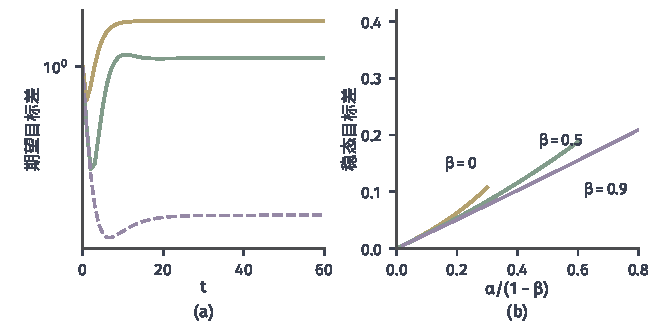
\includegraphics[width=112mm]{figures/05-optimization/05-stochastic-optimization/matplotlib/sgdb-hb-floor/figure.pdf}
  \caption{动量下的噪声残余。(a)贯穿例、$x^{(0)}=2$的期望目标差，由二阶矩的精确递推得到。绿线是$\alpha=0.1$，$\beta=0.5$的重球法；黄线是$\alpha=0.2$的随机梯度下降，有效步长与绿线相同；紫色虚线是$\alpha=0.1$的随机梯度下降。(b)式~\eqref{eq:sgdb-hb-variance}给出的稳态目标差$\frac\lambda2V_0$，$\lambda=2$，$\sigma^2=1$，横轴是有效步长。黄线、绿线、紫线分别取$\beta=0,0.5,0.9$，三条线的$\alpha$都取到$0.3$为止。}
  \label{fig:sgdb-hb-floor}
\end{BookInlineFigure}

\needspace{6\baselineskip}
\paragraph{变量}
\begin{itemize}
 \item $\bm{x}^{(t)}\in\mathbb{R}^n$：当前参数。
 \item $\bm{v}^{(t)}\in\mathbb{R}^n$：速度，形状与参数相同，是算法状态的一部分。
 \item $\hat{\bm g}^{(t)}\in\mathbb{R}^n$：当前点的随机读数。
 \item $\alpha>0$，$0\leq\beta<1$：固定的步长与动量系数。
 \item $T$：预定的总轮数。
\end{itemize}

\paragraph{初始化}
令$\bm{v}^{(0)}=\bm{0}$，第一轮没有历史，与一步随机梯度下降相同。例中是贯穿例的三项一元目标，取$\alpha=0.1$，$\beta=0.5$，读取顺序为第$3,1,2$项，起点和速度是
\[
 x^{(0)}=2,\qquad v^{(0)}=0.
\]

\needspace{6\baselineskip}
\paragraph{每轮更新}
在第$t$轮依次执行：
\begin{enumerate}
 \item \textbf{抽样并读取。}抽取下标$i^{(t)}$，在当前点读取$\hat{\bm g}^{(t)}$。这一步使用的是更新前的位置。例中第一轮抽到第$3$项，
 \[
  \hat g^{(0)}=f_3'(2)=-3.
 \]
 \item \textbf{更新速度。}按式~\eqref{eq:sgdb-hb-velocity}用旧速度和本轮读数计算$\bm{v}^{(t+1)}$。例中第一轮
 \[
  v^{(1)}=0.5\cdot0+(-3)=-3.
 \]
 \item \textbf{更新参数。}用新速度计算$\bm{x}^{(t+1)}$，然后$t\leftarrow t+1$。例中第一轮
 \[
  x^{(1)}=2-0.1\cdot(-3)=2.3.
 \]

 第二轮抽到第$1$项，读数和速度是
 \[
  \hat g^{(1)}=f_1'(2.3)=5.3,\qquad v^{(2)}=0.5\cdot(-3)+5.3=3.8,
 \]
 于是
 \[
  x^{(2)}=2.3-0.38=1.92.
 \]

 第三轮抽到第$2$项，读数和速度是
 \[
  \hat g^{(2)}=f_2'(1.92)=3.84,\qquad v^{(3)}=0.5\cdot3.8+3.84=5.74,
 \]
 于是
 \[
  x^{(3)}=1.92-0.574=1.346.
 \]
\end{enumerate}

单次读数的大小不能作为停止依据，这里按预定轮数结束。例中$T=3$，最终得到$x^{(3)}=1.346$，目标差为$(0.346)^2\approx0.120$。

\paragraph{保证与状态}
随机重球法每轮只多一个$n$维向量和一次向量加法，读取次数不变。恢复运行时必须同时恢复$\bm{v}^{(t)}$：只恢复参数，第一轮就退回了一步无动量的随机梯度下降。

一般目标上的保证要同时限定$\alpha$、$\beta$和读数的条件。定理~\ref{thm:sgdb-hb-variance}只针对二次目标和加性噪声。第~\ref{chap:first-order-methods}章已经看到，重球法在一般强凸光滑目标上，用二次目标的最优参数可能循环；随机读数不会修复这一点。分析时要把$(\bm{x}^{(t)},\bm{v}^{(t)})$作为一个整体，常用的做法是构造同时包含目标差和速度的势函数，递推中的噪声项按所选的势函数进入。

\subsection{随机Nesterov方法}
\label{sec:sgdb-nesterov}

\paragraph{主要思想}
第~\ref{chap:first-order-methods}章的Nesterov方法先沿动量探出去，到探出的位置再求梯度。随机版本的读数也放到这个前瞻点：
\begin{equation}
 \begin{aligned}
 \bm{y}^{(t)}&=\bm{x}^{(t)}+\beta\bigl(\bm{x}^{(t)}-\bm{x}^{(t-1)}\bigr),\\
 \bm{x}^{(t+1)}&=\bm{y}^{(t)}-\alpha\hat{\bm g}^{(t)},
 \end{aligned}
 \label{eq:sgdb-nag}
\end{equation}
这里$\hat{\bm g}^{(t)}$是在$\bm{y}^{(t)}$处读取的。图~\ref{fig:sgdb-state-order}把两种方法的状态次序并排画出。

\begin{BookInlineFigure}
  \centering
  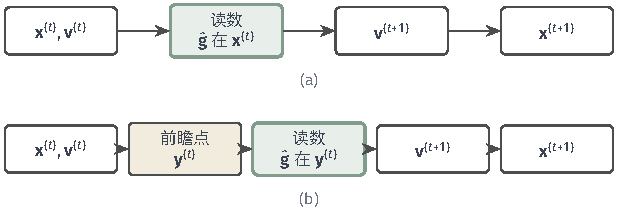
\includegraphics[width=104.64mm]{figures/05-optimization/05-stochastic-optimization/tikz/sgdb-state-order/figure.pdf}
  \caption{一轮内的状态次序。(a)随机重球法在当前点读数，接着更新速度和参数。(b)随机Nesterov方法先用历史算出前瞻点（黄），在前瞻点读数（绿），再更新速度和参数。两种方法的状态都是$(\bm{x}^{(t)},\bm{v}^{(t)})$，读取发生的位置不同。}
  \label{fig:sgdb-state-order}
\end{BookInlineFigure}

$\bm{y}^{(t)}$由抽样之前的量算出，所以固定历史后它是确定的。读数的条件无偏因而写成
\begin{equation}
 \mathbb{E}\bigl[\hat{\bm g}^{(t)}\mid\mathcal{F}^{(t)}\bigr]=\nabla f\bigl(\bm{y}^{(t)}\bigr).
 \label{eq:sgdb-nag-unbiased}
\end{equation}
这里被无偏估计的是前瞻点的梯度，不是$\bm{x}^{(t)}$处的梯度，两者一般不同。下面的比较把这一差别和其他差别列在一起。

\begin{BookInlineTable}
  \centering
  \caption{随机重球法与随机Nesterov方法的比较。}
  \label{tab:sgdb-momentum-compare}
  \begin{tabular}{lll}
    \toprule
    对比项 & 随机重球法 & 随机Nesterov方法\\
    \midrule
    读数位置 & 当前点$\bm{x}^{(t)}$ & 前瞻点$\bm{y}^{(t)}$\\
    条件无偏对象 & $\nabla f(\bm{x}^{(t)})$ & $\nabla f(\bm{y}^{(t)})$\\
    状态 & $\bm{x}^{(t)},\bm{v}^{(t)}$ & $\bm{x}^{(t)},\bm{v}^{(t)}$\\
    一般强凸光滑 & 最优参数可能循环 & 确定性时加速\\
    \bottomrule
  \end{tabular}
\end{BookInlineTable}

贯穿例中取同样的$\alpha=0.1$，$\beta=0.5$，读取顺序仍为第$3,1,2$项。三轮的前瞻点、读数和新位置分别是
\[
 \begin{aligned}
 y^{(0)}&=2, & \hat g^{(0)}&=-3, & x^{(1)}&=2.3,\\
 y^{(1)}&=2.45, & \hat g^{(1)}&=5.45, & x^{(2)}&=1.905,\\
 y^{(2)}&=1.7075, & \hat g^{(2)}&=3.415, & x^{(3)}&=1.366.
 \end{aligned}
\]

第二轮的读数$5.45$是$f_1'$在$y^{(1)}=2.45$处的值，而不是在$x^{(1)}=2.3$处的值。第三轮的前瞻点$1.7075$已经比$x^{(2)}=1.905$更靠近$x^\star=1$，读数相应变小。

\paragraph{方差怎样进入势函数}
确定性的Nesterov方法靠势函数证明加速。把梯度换成带噪声的读数，势函数的递推发生什么变化？下面的定理说明，收缩因子保留，但多了一个不随步数消失的噪声项。记号沿用第~\ref{chap:first-order-methods}章：$q=1/\sqrt\kappa$，以$\bm{u}^{(t)}$表示那里的辅助点。

\begin{theorem}[强凸情形下随机Nesterov方法的势函数递推]
\label{thm:sgdb-nag-noise}
设$f$的梯度$L$-Lipschitz连续且$\mu$强凸，$\mu>0$，最优解为$\bm{x}^\star$。取$\alpha=1/L$，$\beta=(1-q)/(1+q)$，$\bm{x}^{(-1)}=\bm{x}^{(0)}$。设前瞻点的读数满足
\begin{equation}
 \begin{gathered}
 \hat{\bm g}^{(t)}=\nabla f(\bm{y}^{(t)})+\bm{\xi}^{(t)},\\
 \mathbb{E}\bigl[\bm{\xi}^{(t)}\mid\mathcal{F}^{(t)}\bigr]=\bm{0},\qquad
 \mathbb{E}\bigl[\lVert\bm{\xi}^{(t)}\rVert_2^2\mid\mathcal{F}^{(t)}\bigr]\leq\sigma^2.
 \end{gathered}
 \label{eq:sgdb-nag-noise-condition}
\end{equation}
令$\bm{u}^{(0)}=\bm{x}^{(0)}$，并记
\begin{equation}
 \begin{aligned}
 \bm{u}^{(t+1)}&=\bm{x}^{(t)}+\frac1q\bigl(\bm{x}^{(t+1)}-\bm{x}^{(t)}\bigr),\\
 \Phi^{(t)}&=f(\bm{x}^{(t)})-f^\star+\frac\mu2\lVert\bm{u}^{(t)}-\bm{x}^\star\rVert_2^2.
 \end{aligned}
 \label{eq:sgdb-nag-potential}
\end{equation}
则
\begin{equation}
 \mathbb{E}\bigl[\Phi^{(t+1)}\mid\mathcal{F}^{(t)}\bigr]\leq(1-q)\Phi^{(t)}+\frac{\sigma^2}{L},
 \label{eq:sgdb-nag-recursion}
\end{equation}
因而
\begin{equation}
 \mathbb{E}f(\bm{x}^{(T)})-f^\star\leq(1-q)^T\Phi^{(0)}+\frac{\sqrt\kappa\,\sigma^2}{L}.
 \label{eq:sgdb-nag-bound}
\end{equation}
\end{theorem}

\begin{proof}
固定一步，省略上标$(t)$，记$\bm{g}=\nabla f(\bm{y})$，下一步的点记为$\bm{x}^+$和$\bm{u}^+$。

第一步，建立两个恒等式：
\[
 \bm{y}=\frac{\bm{x}+q\bm{u}}{1+q},\qquad
 \bm{u}^+=(1-q)\bm{u}+q\bm{y}-\frac q\mu\hat{\bm g}.
\]
这两个等式只用到更新形式$\bm{x}^+=\bm{y}-\hat{\bm g}/L$，读数是否带噪声不影响代数。第一式在$t=0$时成立，因为$\bm{y}^{(0)}=\bm{u}^{(0)}=\bm{x}^{(0)}$。设第一式对$t$成立，则$q\bm{u}=(1+q)\bm{y}-\bm{x}$，代入第二式右端，并用$q/\mu=1/(qL)$，得到
\[
 \frac1q\bigl(\bm{y}-\tfrac1L\hat{\bm g}-(1-q)\bm{x}\bigr)
 =\bm{x}+\frac1q(\bm{x}^+-\bm{x})=\bm{u}^+ .
\]

再由$\bm{u}^+$的定义和$\beta=(1-q)/(1+q)$，计算
\[
 \frac{\bm{x}^++q\bm{u}^+}{1+q}=\bm{x}^++\frac{1-q}{1+q}(\bm{x}^+-\bm{x})=\bm{y}^{(t+1)},
\]
所以第一式对$t+1$也成立。

第二步，函数项。由下降引理，
\[
 f(\bm{x}^+)\leq f(\bm{y})-\frac1L\langle\bm{g},\hat{\bm g}\rangle+\frac{1}{2L}\lVert\hat{\bm g}\rVert_2^2 .
\]

固定$\mathcal{F}^{(t)}$取条件期望。噪声的条件均值为零，交叉项消失，于是
\[
 \mathbb{E}\hat{\bm g}=\bm{g},\qquad
 \mathbb{E}\lVert\hat{\bm g}\rVert_2^2\leq\lVert\bm{g}\rVert_2^2+\sigma^2 .
\]

代入上式，得到
\[
 \mathbb{E}f(\bm{x}^+)\leq f(\bm{y})-\frac{1}{2L}\lVert\bm{g}\rVert_2^2+\frac{\sigma^2}{2L}.
\]

第三步，距离项。记$\bm{w}=(1-q)\bm{u}+q\bm{y}$，它由历史确定，$\bm{u}^+=\bm{w}-\frac q\mu\hat{\bm g}$。展开平方，用$q^2/(2\mu)=1/(2L)$，取条件期望，得到
\[
 \frac\mu2\mathbb{E}\lVert\bm{u}^+-\bm{x}^\star\rVert_2^2
 \leq\frac\mu2\lVert\bm{w}-\bm{x}^\star\rVert_2^2-q\langle\bm{g},\bm{w}-\bm{x}^\star\rangle+\frac{1}{2L}\bigl(\lVert\bm{g}\rVert_2^2+\sigma^2\bigr).
\]

第四步，相加。两式相加，$\lVert\bm{g}\rVert_2^2$相消，噪声项合计$\sigma^2/L$。剩下的部分完全由历史确定：
\[
 \mathbb{E}\Phi^{(t+1)}\leq f(\bm{y})-f^\star+\frac\mu2\lVert\bm{w}-\bm{x}^\star\rVert_2^2-q\langle\bm{g},\bm{w}-\bm{x}^\star\rangle+\frac{\sigma^2}{L}.
\]

第五步，处理确定部分，与精确梯度时相同。平方范数的凸性给出
\[
 \lVert\bm{w}-\bm{x}^\star\rVert_2^2\leq(1-q)\lVert\bm{u}-\bm{x}^\star\rVert_2^2+q\lVert\bm{y}-\bm{x}^\star\rVert_2^2 .
\]
把$\bm{w}-\bm{x}^\star$写成$(1-q)(\bm{u}-\bm{y})+(\bm{y}-\bm{x}^\star)$，并由强凸性得到
\[
 \langle\bm{g},\bm{y}-\bm{x}^\star\rangle\geq f(\bm{y})-f^\star+\frac\mu2\lVert\bm{y}-\bm{x}^\star\rVert_2^2 .
\]

两式代入后，$\lVert\bm{y}-\bm{x}^\star\rVert_2^2$项抵消，右端成为
\[
 (1-q)\bigl(f(\bm{y})-f^\star\bigr)+(1-q)\frac\mu2\lVert\bm{u}-\bm{x}^\star\rVert_2^2-q(1-q)\langle\bm{g},\bm{u}-\bm{y}\rangle+\frac{\sigma^2}{L}.
\]

第六步，由第一个恒等式，$q(\bm{u}-\bm{y})=\bm{y}-\bm{x}$，所以内积项等于$(1-q)\langle\bm{g},\bm{x}-\bm{y}\rangle$。凸性给出
\[
 \langle\bm{g},\bm{x}-\bm{y}\rangle\leq f(\bm{x})-f(\bm{y}),
\]
于是$f(\bm{y})$消去，得到式~\eqref{eq:sgdb-nag-recursion}。

最后对$t$取全期望并迭代，用$\sum_{j<T}(1-q)^j\leq1/q=\sqrt\kappa$，得到式~\eqref{eq:sgdb-nag-bound}。
\end{proof}

定理的两个条件起不同的作用。条件无偏保证了函数项和距离项中的一次项按精确梯度计算，这是用到式~\eqref{eq:sgdb-nag-noise-condition}第一式的地方。方差界让二次项多出$\sigma^2/(2L)$，函数项和距离项各一份。

与确定性结果的差别在于式~\eqref{eq:sgdb-nag-bound}最后一项。确定性时目标差按$(1-q)^T$收缩到零；有噪声时只能收缩到量级$\sqrt\kappa\sigma^2/L$的邻域，这一项不随$T$消失。所以确定性的加速界不能靠把梯度换成读数直接继承，要进一步下降就要改用更小的步长或增大批量，收缩因子也要随之调整。

式~\eqref{eq:sgdb-nag-bound}是上界，不同方法的上界不宜直接比较。在二次目标上可以写出精确的稳态值。图~\ref{fig:sgdb-accel-noise}用第~\ref{chap:first-order-methods}章的目标$f=(x_1^2+9x_2^2)/2$和起点$(9,1)$比较三种方法。无噪声时，重球法和Nesterov方法远快于梯度下降。加入方差为$1$的加性噪声后，梯度下降、重球法、Nesterov方法的稳态目标差分别约为$0.085$、$0.926$、$0.108$。重球法这组参数的有效步长是$1/3$，大于梯度下降的$1/9$；更重要的是$\lambda=9$时$\alpha\lambda=2.25$，已接近稳定边界$2(1+\beta)=2.5$，式~\eqref{eq:sgdb-hb-variance}的分母很小，噪声残余被放大约$11$倍。Nesterov方法的残余低于定理的上界$\sqrt\kappa\sigma^2/L=1/3$。

\begin{BookInlineFigure}
  \centering
  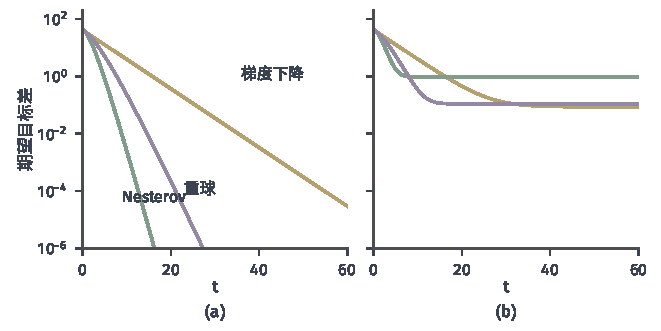
\includegraphics[width=112mm]{figures/05-optimization/05-stochastic-optimization/matplotlib/sgdb-accel-noise/figure.pdf}
  \caption{目标$f=(x_1^2+9x_2^2)/2$，起点$(9,1)$，由二阶矩的精确递推得到的期望目标差。(a)无噪声。(b)读数加上各分量方差为$1$的独立噪声。黄线是$\alpha=1/9$的梯度下降，绿线是$\alpha=\beta=1/4$的重球法，紫线是$\alpha=1/9$，$\beta=1/2$的Nesterov方法。加速缩短了初始阶段，重球法的稳态残余明显更高。}
  \label{fig:sgdb-accel-noise}
\end{BookInlineFigure}

\subsection{Lion符号动量（补充）}
\label{sec:sgdb-lion}

\paragraph{算法}
前两种方法的方向都保留读数的幅度。Lion只取方向的符号：把动量和本轮读数组成候选方向，逐坐标取符号，再按固定步长移动\scite{chen2023lion}。记$\operatorname{sign}(\cdot)$逐坐标作用。取$\bm{m}^{(0)}=\bm{0}$，系数$\beta_1,\beta_2\in[0,1)$，收缩系数$\gamma\geq0$，每轮读取$\hat{\bm g}^{(t)}$后依次计算候选方向和参数更新：
\begin{equation}
 \begin{aligned}
 \bm{c}^{(t)}&=\beta_1\bm{m}^{(t)}+(1-\beta_1)\hat{\bm g}^{(t)},\\
 \bm{x}^{(t+1)}&=\bm{x}^{(t)}-\alpha\operatorname{sign}\bigl(\bm{c}^{(t)}\bigr)-\alpha\gamma\bm{x}^{(t)}.
 \end{aligned}
 \label{eq:sgdb-lion}
\end{equation}

候选方向只参与这一步，下一轮用的动量由另一个系数单独记录：
\begin{equation}
 \bm{m}^{(t+1)}=\beta_2\bm{m}^{(t)}+(1-\beta_2)\hat{\bm g}^{(t)}.
 \label{eq:sgdb-lion-memory}
\end{equation}
$\beta_1$决定当前方向里旧动量占多少，$\beta_2$决定动量本身记忆多长，常见取值是$\beta_1=0.9$，$\beta_2=0.99$。因此读数在方向里的权重是$1-\beta_1$，在历史中的权重却是$1-\beta_2$，两者分开调节。

\paragraph{舍弃幅度}
符号操作舍弃了幅度。设候选方向是$\bm{c}=(0.1,3)$，同向但两个坐标相差$30$倍，取符号后是$(1,1)$，两个坐标移动相同的距离。图~\ref{fig:sgdb-lion-sign}(a)对比了这一点。优点是位移的大小完全由步长决定，读数的尺度和离群值都不会放大位移；缺点是信息少了，当前读数是否接近零，算法并不知道。

\begin{BookInlineFigure}
  \centering
  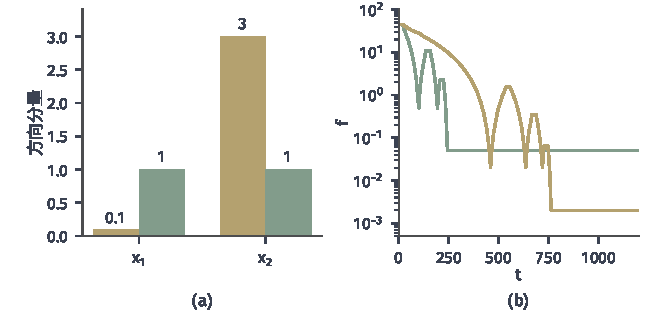
\includegraphics[width=112mm]{figures/05-optimization/05-stochastic-optimization/matplotlib/sgdb-lion-sign/figure.pdf}
  \caption{符号方向的效果。(a)候选方向$(0.1,3)$（黄）与其符号$(1,1)$（绿）。(b)目标$f=(x_1^2+9x_2^2)/2$上$\gamma=0$的Lion，使用精确梯度，纵轴是最近$20$轮内$f$的最大值。绿线$\alpha=0.1$，黄线$\alpha=0.02$。下降段之后曲线不再改善，平台高度随步长变化。}
  \label{fig:sgdb-lion-sign}
\end{BookInlineFigure}

\paragraph{贯穿例的三轮}
取$\alpha=0.1$，$\beta_1=0.9$，$\beta_2=0.99$，$\gamma=0$，$x^{(0)}=2$，$m^{(0)}=0$，读取顺序仍为第$3,1,2$项。三轮的读数、候选方向、新位置和新动量依次是
\[
 \begin{aligned}
 \hat g^{(0)}&=-3, & c^{(0)}&=-0.3, & x^{(1)}&=2.1, & m^{(1)}&=-0.03,\\
 \hat g^{(1)}&=5.1, & c^{(1)}&=0.483, & x^{(2)}&=2.0, & m^{(2)}&=0.0213,\\
 \hat g^{(2)}&=4, & c^{(2)}&=0.419, & x^{(3)}&=1.9, & m^{(3)}&=0.0611.
 \end{aligned}
\]

第一轮的候选方向由反向读数决定，参数上升；此后两轮都下降。读数的大小从$3$变到$5.1$，每轮的位移却都是$0.1$。

\paragraph{分别核对三个量}
第一个量是实际位移：$\gamma=0$时每个坐标的位移大小恰好是$\alpha$（候选方向该坐标非零时），不随读数减小。第二个量是原目标的残差。以$\beta_1=0$的一元精确梯度为例，每步的位移都是$\alpha$，迭代最后在距$x^\star$不超过$\alpha$的范围内来回，残差不会趋于零；$\beta_1>0$时候选方向有滞后，来回的范围由动量决定，同样不会随步数消失。图~\ref{fig:sgdb-lion-sign}(b)取$\beta_1=0.9$，$\beta_2=0.99$，平台的最高值在$\alpha=0.1$时是$0.05$，在$\alpha=0.02$时是$0.002$，减小残差要靠减小步长。

第三个量是参数收缩。$\gamma$项按更新前的参数做收缩，独立于读数和符号。它把参数往原点拉，不是原目标的下降方向，所以残差要按原目标$f$计算，不能把含收缩的位移当成$f$的下降。

\subsection{Muon矩阵动量（补充）}
\label{sec:sgdb-muon}

\paragraph{问题：把矩阵动量变换成更新方向}
参数是矩阵$\bm{W}\in\mathbb{R}^{m\times d}$时，动量$\bm{B}$也是矩阵。Lion逐元素地把幅度抹去，Muon在奇异方向上做类似的事：保留动量的奇异向量，把奇异值全部变成$1$\scite{jordan2024muon}。

这正是极分解所做的。矩形矩阵$\bm{B}$的紧奇异值分解是$\bm{B}=\bm{U}\bm{\Sigma}\bm{V}^\top$，极分解把它写成部分等距与半正定因子之积，
\begin{equation}
 \bm{B}=\bm{U}\bm{V}^\top\cdot\bm{V}\bm{\Sigma}\bm{V}^\top,\qquad
 \operatorname{orth}(\bm{B})=\bm{U}\bm{V}^\top .
 \label{eq:sgdb-polar}
\end{equation}
这里$\bm{U}\bm{V}^\top$就是\term{极因子}（polar factor），奇异向量与$\bm{B}$相同，奇异值全部是$1$。极分解的存在性和唯一性条件可参考\BookChapterRef{chap:polar-decomposition}{卷二第8章“极分解”}。

奇异值分解太贵，Muon用矩阵多项式的有限次迭代来近似极因子。设$\bm{X}=\bm{U}\bm{\Sigma}\bm{V}^\top$，对奇次多项式$p(\sigma)=\sum_jc_j\sigma^{2j+1}$，有
\begin{equation}
 \sum_jc_j\bm{X}\bigl(\bm{X}^\top\bm{X}\bigr)^j=\bm{U}\,p(\bm{\Sigma})\,\bm{V}^\top ,
 \label{eq:sgdb-odd-poly}
\end{equation}
所以这样的迭代不改变奇异向量，只对每个奇异值作用多项式。于是问题变成：选$p$，使得多次复合后所有奇异值都接近$1$。

\paragraph{算法次序}
一次更新的次序是：
\begin{enumerate}
 \item \textbf{读取。}在当前点（或前瞻点）得到矩阵读数$\hat{\bm G}^{(t)}$。
 \item \textbf{更新动量。}用旧动量和本轮读数计算
 \begin{equation}
  \bm{B}^{(t+1)}=\beta\bm{B}^{(t)}+\hat{\bm G}^{(t)}.
  \label{eq:sgdb-muon-momentum}
 \end{equation}
 \item \textbf{归一化。}用Frobenius范数除以动量，得到
 \[
  \bm{X}_0=\frac{\bm{B}^{(t+1)}}{\lVert\bm{B}^{(t+1)}\rVert_{\mathrm{F}}},
 \]
 所有非零奇异值落到$(0,1]$。
 \item \textbf{有限次迭代。}按多项式迭代$k$次，得到$\bm{X}_k$。
 \item \textbf{更新参数。}$\bm{W}^{(t+1)}=\bm{W}^{(t)}-\alpha\bm{X}_k$。
\end{enumerate}

经典的Newton--Schulz迭代取$p(\sigma)=\frac12(3\sigma-\sigma^3)$，矩阵形式是
\begin{equation}
 \bm{X}_{j+1}=\frac32\bm{X}_j-\frac12\bm{X}_j\bm{X}_j^\top\bm{X}_j .
 \label{eq:sgdb-newton-schulz}
\end{equation}
这个$p$有不动点$\sigma=1$，导数$p'(1)=0$，所以在$1$附近二阶收敛；对$\sigma\in(0,1]$迭代单调上升到$1$，起点离零很近时每步只放大约$1.5$倍。归一化保证了奇异值落在收敛区域里。

\paragraph{理想极因子与有限步近似}
用具体矩阵计算。取
\[
 \bm{B}=\begin{bmatrix}3&1\\1&3\end{bmatrix}.
\]
它的奇异值是$4,2$，奇异向量相同，极因子是单位矩阵$\bm{I}$。按Frobenius范数$\sqrt{20}$归一化后，奇异值是
\[
 0.894,\qquad 0.447.
\]

由式~\eqref{eq:sgdb-newton-schulz}迭代一次，两个奇异值变成$0.984$和$0.626$；迭代三次是$1.000$和$0.953$；迭代五次是$1.000$和$0.99998$，已经非常接近理想的极因子$\bm{I}$。图~\ref{fig:sgdb-muon-singular}(a)画出一般的$\sigma$：奇异值越小，需要的迭代次数越多。

\begin{BookInlineFigure}
  \centering
  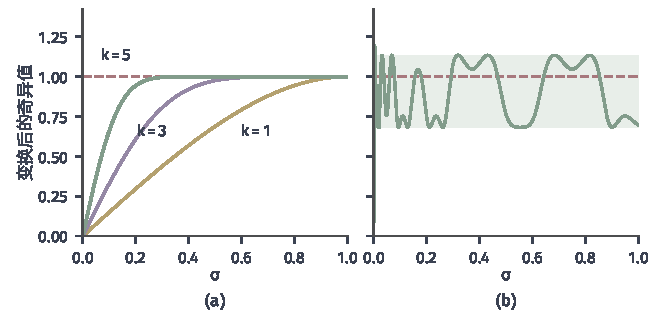
\includegraphics[width=112mm]{figures/05-optimization/05-stochastic-optimization/matplotlib/sgdb-muon-singular/figure.pdf}
  \caption{有限次迭代对奇异值的作用，横轴是归一化后的奇异值，红色虚线是理想的$1$。(a)经典Newton--Schulz迭代$k=1,3,5$次。(b)五次多项式$3.4445\sigma-4.7750\sigma^3+2.0315\sigma^5$复合$5$次，绿底是$\sigma\in[0.02,1]$上的取值范围，约为$[0.68,1.13]$。}
  \label{fig:sgdb-muon-singular}
\end{BookInlineFigure}

实际实现常用五次多项式\scite{jordan2024muon}：
\begin{equation}
 p(\sigma)=3.4445\,\sigma-4.7750\,\sigma^3+2.0315\,\sigma^5 .
 \label{eq:sgdb-muon-poly}
\end{equation}
它的系数是为“只迭代五次”专门选的。$p(1)=0.701$，$\sigma=1$不是它的不动点，继续迭代不会收敛到极因子。它的优势是小奇异值被放大得更快：在图~\ref{fig:sgdb-muon-singular}(b)中，$\sigma\in[0.02,1]$上五次复合后的值都落在约$[0.68,1.13]$内。

上面的矩阵用五次多项式迭代五次，奇异值变成$1.114$和$0.689$，与理想值$1$差得较远；两个奇异值之比从$2$缩小到约$1.6$。所以$\bm{X}_k$是对动量的尺度压缩，而不是精确的极因子。

\paragraph{计算成本与含义}
设$m\geq d$，先把$\bm{X}^\top\bm{X}$算出来。每次迭代做一次$\bm{X}^\top\bm{X}$、一次$(\bm{X}^\top\bm{X})^2$和一次$\bm{X}$右乘，运算量是$O(md^2)$；迭代$k$次合计$O(kmd^2)$。完整的奇异值分解也是这个量级，但常数更大。比较方法时，这部分要计入，每步的读取次数不变不等于每步成本不变。

动量矩阵和它的变换都只由梯度读数算出，其中没有二阶导数。奇异值变成$1$是对历史读数的幅度处理，它不是目标Hessian的近似。这种方法在什么问题上有效，只能在具体问题上由实际的目标值或验证指标判断。
